\documentclass[t, screen, aspectratio=43]{beamer}
\usepackage[T1]{fontenc}
\usepackage[utf8]{inputenc}
\usepackage{epsf}
\usepackage{graphicx}
\usepackage{geometry}
\usepackage{tabularx}
\usepackage[table]{colortbl}
\usepackage{xcolor}
\usepackage{soul}
\usepackage[normalem]{ulem}
% Use the NTNU-temaet for beamer 
% \usetheme[style=ntnu|simple|vertical|horizontal, 
%     language=bm|nn|en, 
%     smalltitle, 
%     city=all|trondheim|alesund|gjovik]{ntnu2017}
\usetheme[style=helvet,language=en]{ntnu2017}

\usepackage[english]{babel}
\usepackage[style=numeric,backend=biber,natbib=false,sorting=none]{biblatex}

\title[Short title]{Ultra-Low Power PLL for Wake-up Receiver Applications}
\subtitle{Specialization Project Progress - 6th Week}
\author[C Nielsen]{Cole Nielsen}
\institute[NTNU]{Department of Electronic Systems, NTNU}
\date{4 October 2019 (Calendar week 40)}
%\date{} % To have an empty date

\addbibresource{example.bib} % Add bibliography database

% Set the reference style to numeric.
% See here: http://tex.stackexchange.com/questions/68080/beamer-bibliography-icon
\setbeamertemplate{bibliography item}[text] 

% Set bibliography fonts to a small size.
\renewcommand*{\bibfont}{\footnotesize}

\begin{document}

\begin{frame}
	\titlepage%
\end{frame}

% Alternatively, special title page command to get a different background
% \ntnutitlepage

% #############################################################################
% Timeline
% #############################################################################
\begin{frame}
	\frametitle{Autumn Timeline}
	\begin{table}[htb!]
		\tiny
		\centering
		\vspace{-1em}
		\def\arraystretch{1.5}		
		\setlength\arrayrulewidth{0.75pt}
		\setlength{\tabcolsep}{1em} % for the horizontal padding
		\begin{tabular}{|l|l|l|l|}
			\hline 
			\rule[-1ex]{0pt}{2.5ex} \cellcolor{gray!40}\textbf{Week} & \cellcolor{gray!40}\textbf{Dates} &\cellcolor{gray!40}\textbf{Tasks} & \cellcolor{gray!40}\textbf{Outcomes}\\ 
			\hline 
			\rule[-1ex]{0pt}{2.5ex} \cellcolor{red!20}\textbf{36}& \cellcolor{red!20}2.9 - 8.9 & \cellcolor{red!20}Review PLL Design & \cellcolor{red!20}Refreshed Knowledge\\ 
			\hline 
			\rule[-1ex]{0pt}{2.5ex} \cellcolor{red!20}\textbf{37}& \cellcolor{red!20}9.9 - 15.9 & \cellcolor{red!20}Modeling/simulation (set up) & \cellcolor{red!20}--\\ 
			\hline 
			\rule[-1ex]{0pt}{2.5ex} \cellcolor{red!20}\textbf{38}& \cellcolor{red!20}16.9 - 22.9 & \cellcolor{red!20}Modeling/simulation &\cellcolor{red!20} TDC/DCO Requirements\\ 
			\hline 
			\rule[-1ex]{0pt}{2.5ex} \cellcolor{red!20}\textbf{39}& \cellcolor{red!20}23.9 - 29.9& \cellcolor{red!20}Modeling/simulation& \cellcolor{red!20}Loop Filter/Digital Algorithms\\ 
			\hline 
			\rule[-1ex]{0pt}{2.5ex} \cellcolor{green!20}\textbf{40}& \cellcolor{green!20}30.9 - 6.10& \cellcolor{green!20}Modeling/simulation& \cellcolor{blue!20}\color{red}{\textbf{Loop filter, DCO, TDC, calibration}}\color{black}\\ 
			\hline 
			\rule[-1ex]{0pt}{2.5ex} \textbf{41}& 7.10 - 13.10& Circuit Research &\cellcolor{blue!20} DCO/Divider topologies, \color{red}\textbf{Ideal Virtuoso implementation}\\ 
			\hline 
			\rule[-1ex]{0pt}{2.5ex} \textbf{42}& 14.10 - 20.10& Circuit Research & TDC/other topologies\\ 
			\hline 
			\rule[-1ex]{0pt}{2.5ex} \textbf{43}& 21.10 - 27.10& Circuit Implementation& Digital logic (schematic)\\ 
			\hline 
			\rule[-1ex]{0pt}{2.5ex} \textbf{44}& 28.10 - 3.11& Circuit Implementation& DCO (schematic)\\ 
			\hline 
			\rule[-1ex]{0pt}{2.5ex} \textbf{45}& 4.11 - 10.11& Circuit Implementation& Divider/other (schematic)\\ 
			\hline 
			\rule[-1ex]{0pt}{2.5ex} \textbf{46}& 11.11 - 17.11& Circuit Implementation (TDC)& \\ 
			\hline 
			\rule[-1ex]{0pt}{2.5ex} \textbf{47}& 18.11 - 24.11& Circuit Implementation (TDC)& TDC (schematic)\\ 
			\hline 
			\rule[-1ex]{0pt}{2.5ex} \textbf{48}& 25.11 - 1.12& Full Circuit testing & Testbenches, find bugs, design fixes\\ 
			\hline 
			\rule[-1ex]{0pt}{2.5ex} \textbf{49}& 2.12 - 8.12& Full Circuit testing& Design Fixes/iteration\\ 
			\hline 
			\rule[-1ex]{0pt}{2.5ex} \textbf{50}& 9.12 - 15.12& --& --\\ 
			\hline 
		\end{tabular}
		\begin{flushleft}\textbf{Legend:} \colorbox{red!20}{\textbf{Done}} \colorbox{green!20}{\textbf{Current}}  \colorbox{blue!20}{\textbf{Revised}}
		% *I will write the report simultaneously with the work.
		\end{flushleft}
		% \caption{Assigned specifications for branch line hybrid design.}
		% \label{asgn_specs}
	\end{table}   
\end{frame}


% #############################################################################
% This week
% #############################################################################

\begin{frame}
	\frametitle{Timeline Tasks}
	\begin{block}{This week}
		\begin{itemize}
			\footnotesize
			\item Originally planned on implementing ideal simulation in Virtuoso using ideal library components and some Verilog.
			\item \textit{What I actually did}:
			\begin{itemize}
				\footnotesize
				\item Found issue with how I defined phase noise requirements
					\begin{itemize}
						\scriptsize
						\item Had to redefine this, the TDC and loop bandwidth specification.
					\end{itemize}
				\item Had to rework DCO simulation model to have accurate phase noise.
				\item Analyzed sensitivity/variation of DCO gain for loop filter analysis.
				\item Analyzed TDC to determine accuracy/linearity (tied to calibration)
				\item Decided to change loop filter to use PI-based control.
			\end{itemize} 
		\end{itemize}    
	\end{block}
\end{frame}

% #############################################################################
% sim/modeling approach
% #############################################################################

\begin{frame}
	\frametitle{Requirements redefinition}
	\begin{block}{Redefining phase noise and loop bandwidth requirements}
		\begin{itemize}
			\scriptsize
			\item \textit{Made bad assumption with original requirements}, i.e. residual frequency modulation is predicated on a Gaussian phase noise distribution.
			\item Now redefined in terms of the actual spectum of the PLL for use with 2FSK. Phase noise is derived from the closed loop PLL transfer function G(f).
			\item Bandwidth is now selected to minimize amount of power that overlaps in 2FSK tones.
			\begin{itemize}
				\scriptsize
				\item (Integrated PSD in overlap)/(total power) = bit error probability.
			\end{itemize}
			\vspace{-0.5em}
			\center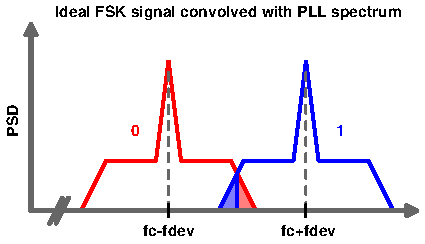
\includegraphics[width=0.4\textwidth, angle=0]{fsk_tones_rx2.pdf}
			\vspace{-0.5em}
		\end{itemize} 	
	\end{block}
\end{frame}

\begin{frame}
	\frametitle{Requirements redefinition}
	\begin{block}{Loop definition and phase noise components.}
		% \vspace{-.2em}
		\begin{minipage}{7cm}
			\vspace{1em}
			\begin{itemize}
				\scriptsize
				\item Phase noise and closed loop response G(f) are simple to define. Second order butterworth G(f) is desired. Loop bandwidth = $\omega_N$, $\zeta$ = 0.707:
				\tiny
				\begin{equation}
					G(f) = \frac{\omega_N^2}{s^2 + 2\zeta\omega_n s + \omega_N^2}
				\end{equation}
				\scriptsize
				\item The TDC quantization phase noise is given by: 
				\tiny
				\begin{equation}
					PN_{TDC}(f) = f_{ref}\cdot|2\pi NG(f)|^2\cdot \frac{\Delta t_{del}^2}{12}
				\end{equation}
				\scriptsize	
				\item The oscillator phase noise (based on ring oscillator theoretical limit) is: 
				\tiny
				\begin{equation}
					PN_{osc}(f) = |1-G(f)|^2\cdot  \frac{7.33 k_B T}{P_{osc}}\cdot\left(\frac{f_0}{f}\right)^2
				\end{equation}
				\scriptsize	
			\end{itemize}  

		\end{minipage}%
		% \hspace{-0.5cm}
		\begin{minipage}{5cm}
			% \vspace{-1.5em}
			\center
			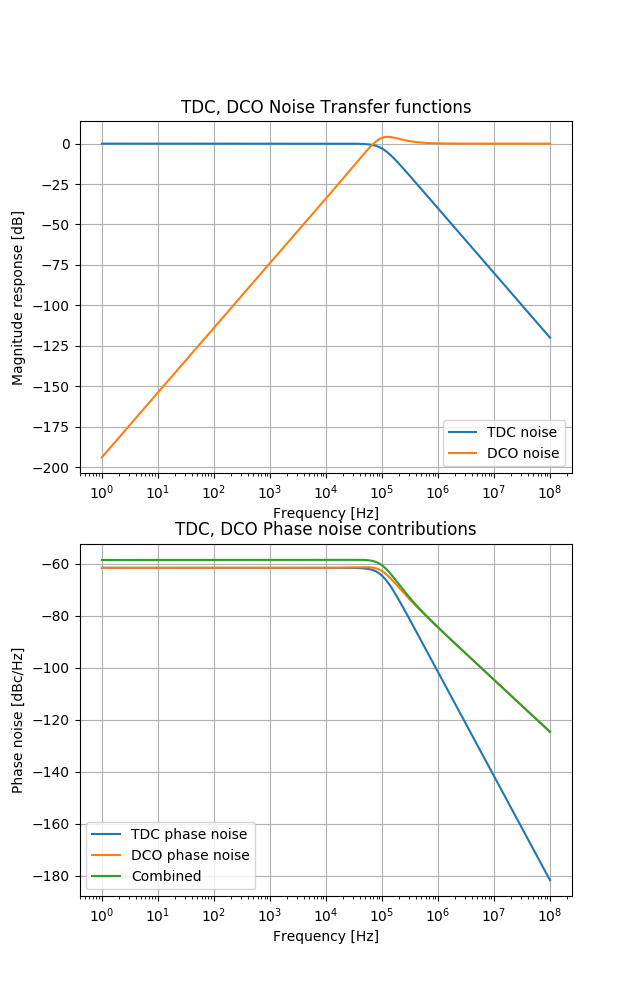
\includegraphics[width=0.8\textwidth, angle=0]{phase_noise_curves.png}
			% \vspace{-0.5em}  
		\end{minipage}%
	\end{block}
\end{frame}

\begin{frame}
	\frametitle{Requirements redefinition}
	\begin{block}{Connecting BER, loop bandwidth, frequency deviation.}
		\begin{itemize}
			\scriptsize
			\item  Need to calculate power of oscillator within $\Delta f$ of the carrier. If $V_{osc} = \Re\left(e^{j\omega_0t - j\phi_{noise}(t)}\right)$, and $\phi_{noise}(t)$ is small:
			\tiny
			\begin{equation}
				\Re\left(e^{j\omega_0t - j\phi_{noise}(t)}\right) \approx \Re\left(e^{j\omega_0t}(1-j\phi_{noise}(t))\right) = \cos(\omega_0t) + \phi_{noise}(t)\sin(\omega_0t)
			\end{equation}
			\scriptsize	
			\item  The power within $\Delta f$ of the carrier is (if the carrier is normalized to a power of 1):
			\tiny
			\begin{equation}
				P_{out}(\Delta f) = 1 + 2\int_0^{\Delta f}\phi_{noise}^2(t)df
			\end{equation}
			\scriptsize	
			\item To find the minimum FSK frequency deviation for a given BER, the following is solved computationally. This is based on the overlap principle. ($f_{dev}=\Delta f$)
			\tiny
			\begin{equation}
				P_{out}(\Delta f=\infty)\cdot(1-2BER) = 1 + 2\int_0^{f_{dev}}\phi_{noise}^2(t)df
			\end{equation}
		\end{itemize} 	
	\end{block}
\end{frame}


\begin{frame}
	\frametitle{Requirements redefinition}
	\begin{block}{Solving for loop bandwidth computationally}
		\begin{itemize}
			\scriptsize
			\item Most power from phase noise is accumulated near frequency of loop bandwidth.
			\item TDC and DCO noise were optimized to provide approximately the same contribution to phase noise.
			\item For 250 kHz of frequency deviation, $\leq$ 70 kHz of closed loop bandwidth is required. 
			\item Selecting 50 kHz loop bandwidth, with 64 TDC steps to allow for 50 kHz margin on BER=1e-2 with $f_{dev}$ = 250 kHz.
		\end{itemize}
			\vspace{-0.5em}
			\center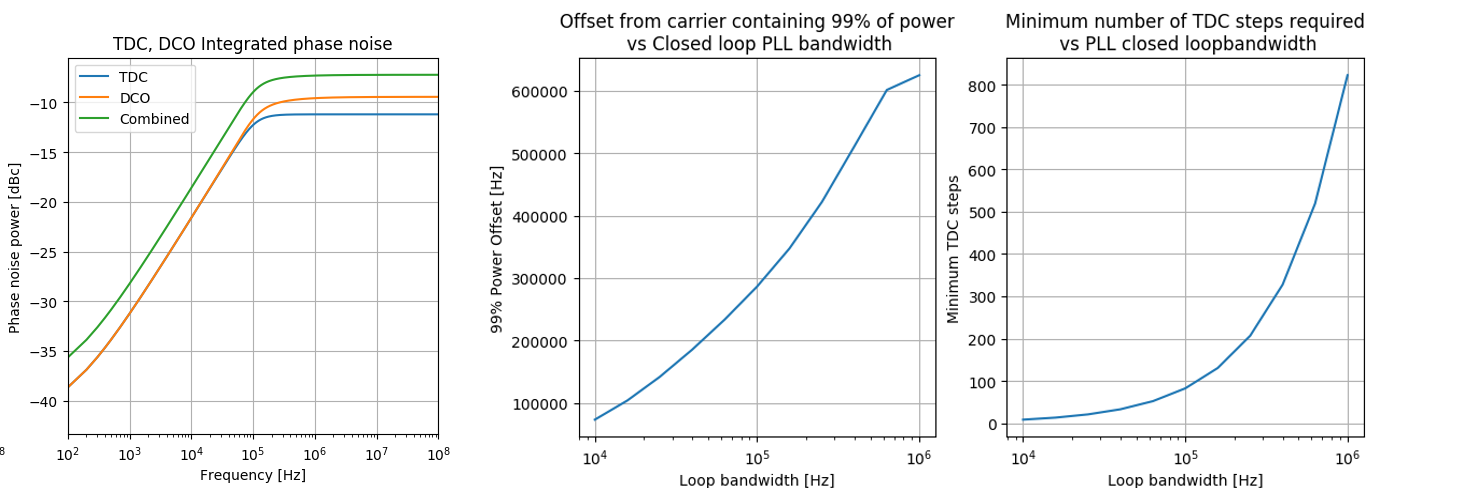
\includegraphics[width=0.8\textwidth, angle=0]{pow_integ.png}
			\vspace{-0.5em} 	
	\end{block}
\end{frame}


\begin{frame}
	\frametitle{Loop Filter}
	\begin{block}{Resolving unknowns}
		\begin{itemize}
			\footnotesize
			\item Thoughtful loop filter design requires consideration of some physical parameters
			\begin{itemize}
				\scriptsize
				\item\textbf{TDC accuracy}
				\begin{itemize}
					\scriptsize
					\item Affects PLL transfer function, so we want to minimize variation.
					\item Innately tied to calibration process.
					\item Important for accurate calibration of frequency, to hit PLL lock-in range.
					\item Important for INL; also DNL associated with TDC phase wrap-over.
				\end{itemize}
				\item \textbf{$K_{DCO}$ and variance of $K_{DCO}$}
				\begin{itemize}
					\scriptsize
					\item Very important in determining gain coeficients in loop filter.
					\item Variance of $K_{DCO}$ will be \textbf{the most} significant factor in overall PLL loop perfomance variation, and will be hard to calibrate.
					\item 
				\end{itemize}
			\end{itemize}
			\item Consequently, I analyzed the real-hardware considerations for these parameters to provide some inside into the loop design. 
		\end{itemize} 	
	\end{block}
\end{frame}


\begin{frame}
	\frametitle{TDC accuracy}
	\begin{block}{Resolving unknowns}
		\begin{itemize}
			\scriptsize
			\item Had to look into TDC circuit architectures to consider question accuracy and calibration.
			\item \textbf{Analog or digital??}
			\begin{itemize}
				\scriptsize
				\item \textbf{Analog}
				\begin{itemize}
					\scriptsize
					\item (+) Better accuracy (always running)?
					\item (-) Constant Power draw from CP/loop filter
					\item (-) Have to wait for lock everytime
				\end{itemize}

				\item \textbf{Digital}
				\begin{itemize}
					\scriptsize
					\item Calibrate once, run for a long time before recalibrating.
					\item Lower overall power.
					\item Inherent drift.
					\item Possibility - Counter based design requiring no calibration???
				\end{itemize}
			\end{itemize}
			\item Currently believe digital will have power supremacy.
			\item Targeting $\pm$ 50 ppm accuracy to correspond to $\pm$ 120 kHz at 2.4 GHz.
		\end{itemize} 	
	\end{block}
\end{frame}

\begin{frame}
	\frametitle{Analog TDC}
	\begin{block}{Traditional Analog DLL}
		\begin{minipage}{7cm}
		\vspace{1em}
		\begin{itemize}
			\scriptsize
			\item Simple analog DLL with M inverter stagers, first order filter.
			\item Lock time on the order of 10 $ \mu$s. With digital, amortized calibration time \textbf{should} be much lower than this.
			\item With first order loop filter, 9.9$\cdot\tau$ is required for $\pm$ 50 ppm settling.
			\begin{itemize}
				\scriptsize
				\item For 10 $ \mu$s settling time, given $t_{settled} = 9.2/(2\pi f_p) \rightarrow f_p = 157$ kHz.
			\end{itemize}
			\item with $2^N$=M stages, tap stages M/2 ($\bar{I}$), 3M/4($\bar{Q}$) and M ($I$) to use simple IQ based charge pump/phase detector circuit on the right.
		\end{itemize} 	
		\end{minipage}%
		% \hspace{-0.5cm}
		\begin{minipage}{5cm}
		\center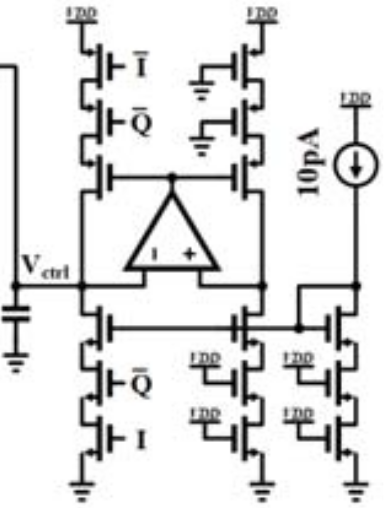
\includegraphics[width=0.6\textwidth, angle=0]{cp_lf.png}
		\end{minipage} 
	\end{block}
\end{frame}

\begin{frame}
	\frametitle{Digital TDC}
	\begin{block}{Calibrated Delay line}
			\vspace{-0.5em}
			\center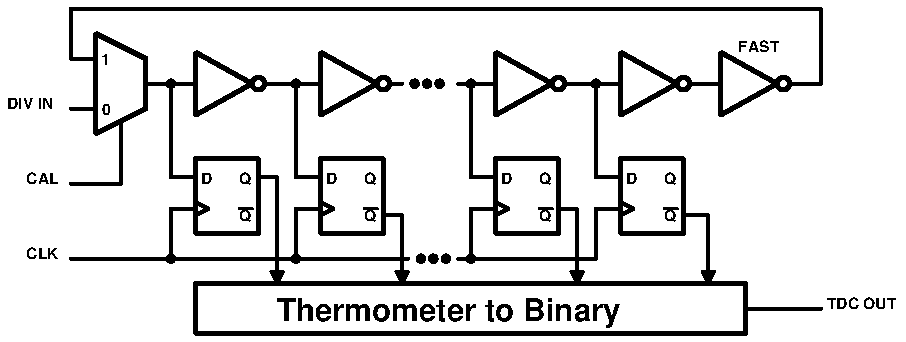
\includegraphics[width=0.5\textwidth, angle=0]{tdc_cal.pdf}	
		\begin{itemize}
			\scriptsize
			\item Standard M-stage inverter-based delay line.
			\item Use mux to allow for delay line to operate as ring oscillator
			\item Measure phase with TDC of free-running oscillator.
			\begin{itemize}
				\scriptsize
				\item Change in phase between measurements is related to error of the delay line.
			\end{itemize}
			\item If $\Delta t_{line}$ is the delay error of the delay line:
			\tiny
			\begin{equation}
				\frac{\Delta t_{line}}{T_{ref}} = \frac{\Delta TDC(N_{CYCLES})}{M\cdot N_{CYCLES}}
			\end{equation}
			\scriptsize	
		\end{itemize}

	\end{block}
\end{frame}


\begin{frame}
	\frametitle{Digital TDC - Algorithm}
	\begin{block}{Calibrated Delay line}
		\begin{itemize}
			\scriptsize

			\item For $\pm$ 50 ppm accuracy, 10\% tuning range and 10-bit DAC is sufficient.
			\item Use binary search algorithm to find optimal tuning word.
			\begin{itemize}
				\scriptsize
				\item Frequency measurement granularity increases with measurement period, start coarse and increase double time with step of binary search
			\end{itemize}		
			\item With M=64, and 10 bits, search will take 128 $\mu$s. 
			\item(May also require some coarse calibration, this is expected to be fast)
			\item Better than analog if we calibrate less than 1 in 13 power ups.
			\begin{itemize}
				\scriptsize
				\item 40 power-ups a second with 10 sec between calibrations this is amortizes to 0.32 $\mu$s  calibration time per wake up. 
			\end{itemize}				
		\end{itemize} 	
	\end{block}
\end{frame}

\begin{frame}
	\frametitle{Digital TDC}
	\begin{block}{Counter-based TDC}
			\vspace{-0.5em}
			\center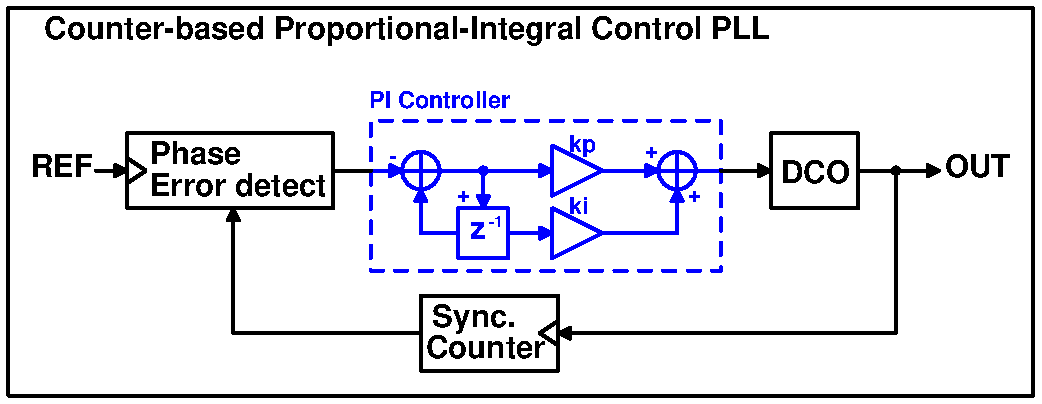
\includegraphics[width=0.5\textwidth, angle=0]{counter_pll.pdf}	
		\begin{itemize}
			\footnotesize
			\item Use synchronous counter clocked by oscillator to keep track of phase.
			\item Loop filter samples the counter phase every reference clock cycle.
			\item \textbf{Requires no calibration.} Linearity good.
			\item Resolution is $\log_2(2.4G/16M)$ = 7.2 bits. Good enough. 
			\item Instant start up.
			\item \color{red} \textbf{Power will be an issue???}
			\item \color{black} Will have to test in simulation...
		\end{itemize} 	
	\end{block}
\end{frame}

\begin{frame}
	\frametitle{DCO frequency tuning and $K_{DCO}$}
	\begin{block}{Resolving unknowns}
		\begin{itemize}
			\scriptsize
			\item The fractional tuning range of the oscillator is:
			\tiny
	\begin{equation}
		\frac{\Delta f}{f_c} = \frac{1}{2}\cdot\frac{\gamma V_{DD}\left( 1-\ln2 \right)}{V_{DD}\left(\frac{7}{8}-\ln2+\frac{\gamma}{2}-\frac{\gamma}{2}\ln2\right)-V_{t0}\left(1-\ln2\right)}
	\end{equation}	
			\scriptsize
			\item If a N-bit DAC is used to control the oscillator, the resulting DCO gain is therefore:
			\tiny
	\begin{equation}
		K_{DCO} = \frac{\Delta f}{2^{N_{DAC}}} = \frac{f_c}{2^{N_{DAC}+1}}\cdot\frac{\gamma V_{DD}\left( 1-\ln2 \right)}{V_{DD}\left(\frac{7}{8}-\ln2+\frac{\gamma}{2}-\frac{\gamma}{2}\ln2\right)-V_{t0}\left(1-\ln2\right)}
	\end{equation}	
			\scriptsize
			\item The variation of the DCO gain, given the parameters it depends on is:
			\tiny
	\begin{equation}
		\sigma_{KDCO} = \sqrt{\left(\frac{\partial K_{DCO}}{\partial V_{DD}}\cdot\frac{\sigma_{VDD}}{K_{DCO}} \right)^2 + \left(\frac{\partial K_{DCO}}{\partial V_{t0}}\cdot\frac{\sigma_{Vt0}}{K_{DCO}} \right)^2 + \left(\frac{\partial K_{DCO}}{\partial \gamma}\cdot\frac{\sigma_\gamma}{K_{DCO}} \right)^2}
	\end{equation}
			\scriptsize
			\item For example: 1\% variation in all parameters yields ca. 6\% variation in tuning.
		\end{itemize} 	
	\end{block}
\end{frame}

\begin{frame}
	\frametitle{DCO fix}
	\begin{block}{Updating phase noise model}
		\begin{itemize}
			\scriptsize
			\item Fixed phase noise model in time domain simulation of PLL.
			\item Before phase noise was not accurately set, just loosely.
			\item Derived a Z-domain model for discrete random phase walk, am able now to convert continuous time phase noise spec to a discrete time model with accurate phase noise.
		\end{itemize} 	
	\end{block}
\end{frame}

\begin{frame}
	\frametitle{Loop Filter Change}
	\begin{block}{Change to PID based loop filter}
		\vspace{-0.5em}
		\begin{itemize}
			\scriptsize
			\item \textbf{Old:} Complicated.
		\end{itemize} 	
		\vspace{-1em} 
		\center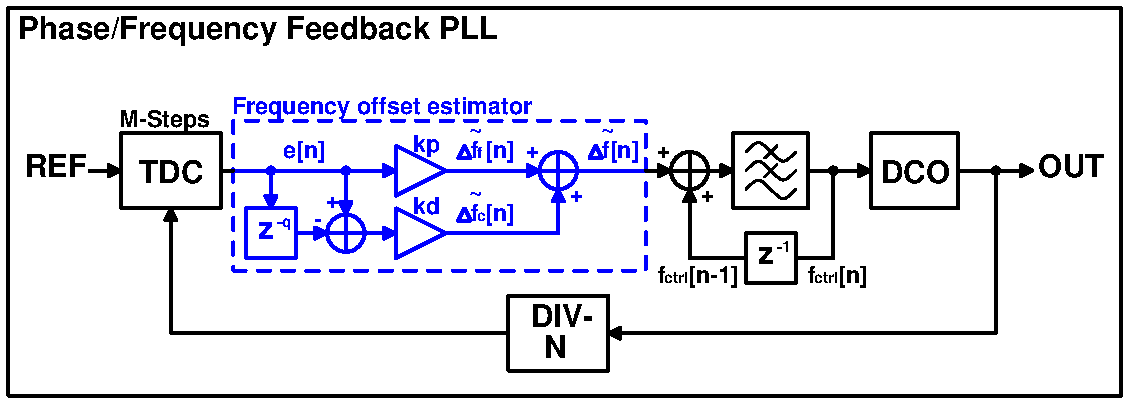
\includegraphics[width=0.5\textwidth, angle=0]{more_advanced.pdf}
		\begin{itemize}
			\scriptsize
			\item \textbf{New:} Much simpler PID-based, added phase accumulator to handle wrap-over issues, allows for more stable control. Calibration should prevent accumulator overflow. Derivative path only used for calibration (not shown).
		\end{itemize}
		\vspace{-1em}
		\center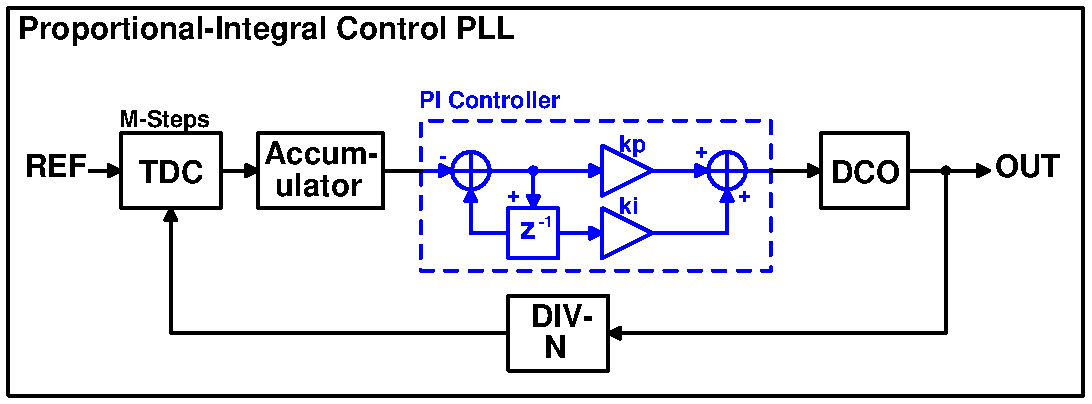
\includegraphics[width=0.5\textwidth, angle=0]{pi_pll.pdf} 
	\end{block}
\end{frame}



\begin{frame}
	\frametitle{Loop Filter}
	\begin{block}{Coarse frequency offset estimation}
		\vspace{-0.5em}
		\center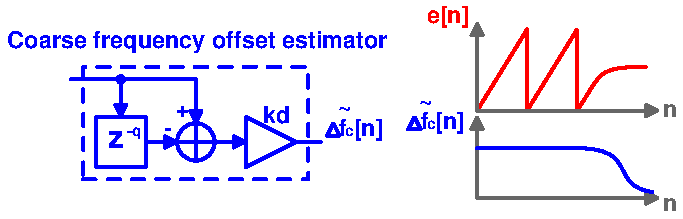
\includegraphics[width=0.5\textwidth, angle=0]{coarse_est.pdf}
		\begin{itemize}
			\footnotesize
			\item \textbf{Coarse frequency estimation:} Given M-step TDC, outputting phase error signal e$_\phi$[n], and a divider modulus N
			\tiny
			\vspace{-1em}
			\begin{equation}
				\Delta \phi_{DCO}[n; q] = N\cdot\Delta \phi_{REF}[n] = 2\pi \frac{N}{M}\left( e_\phi[n]-e_\phi[n-q]\right ),\hspace{2em} \Delta \phi_{DCO}[n; q] = \Delta \omega_{DCO}[n]qT_{ref} = 2\pi q \frac{\Delta \tilde f_{DCO}}{f_{ref}}
			\end{equation}
			\vspace{-1em}
			\begin{equation}
				\Delta \tilde f_{c} =\Delta \tilde f_{DCO} = \frac{f_{ref}}{q}\frac{N}{M}\left( e_\phi[n]-e_\phi[n-q]\right )
			\end{equation}				
			\footnotesize	
			\item Is a discrete differentiator, with gain coeficient to convert $d\phi/dt$ to frequency. 
			\begin{itemize}
				\scriptsize
				\item Design logic to handle phase wrapping.	
				\item Useful in coarse frequency range calibration. Can detect fast if frequency offset too large.
				\item Delay q is used to increase frequency resolution. 
			\end{itemize}			
		\end{itemize} 	
	\end{block}
\end{frame}




\begin{frame}
	\frametitle{Frequency Calibration (New)}
	\begin{block}{Coarse frequency calibration algorithm}
		\begin{itemize}
			\vspace{-0.25em}
			\scriptsize
			\item Use binary search algorithm to tune capacitor bank for frequency range.
			\item With 75 cycles measurement time, 2.4 GHz RF frequency, 16 MHz reference, and 64 TDC steps, within 0.5 MHz can be measured in 5 $\mu$s
			\item A 4 bit binary seach would take circa 20 $\mu$s to execute. 
			\item Should hopefully put initial frequency of PLL in lock range, and avoid issues with phase wrapping in the phase error accumulator.
		\end{itemize} 	
 
	\end{block}
\end{frame}


% #############################################################################
% Loop Dynamics (continuous)
% #############################################################################

% \begin{frame}
% 	\frametitle{Loop Dynamics}
% 	\begin{block}{Still To Do}
% 		\vspace{-.2em}
% 		\begin{itemize}
% 			\footnotesize
% 			\item Standard approach to used mixed continuous/discrete time mathematical model for DPLL. 
% 			\item Plot of RO phase noise (typical)
% 			\item Automatic analysis of performance (lock detection, residual phase modulation, lock-in/pull-in range).
% 			\item Automatic optimization (using gradient descent) of PLL parameters?
% 			\item Z-domain modeling of loop? Develop (by hand) some ideal transfer funtions for loop.

% 		\end{itemize}    
% 	\end{block}
% \end{frame}

% #############################################################################
% Specification
% #############################################################################

\begin{frame}
	\frametitle{Specification \color{red}(changed)\color{black}}
	\begin{block}{System Performance Targets}
		\scriptsize
		\begin{table}[h!]
			\centering
			\def\arraystretch{1.5}		
			\setlength\arrayrulewidth{0.75pt}
			\setlength{\tabcolsep}{1em} % for the horizontal padding
			\begin{tabular}{|l|r|l|l|}
				\hline 
				\rule[-1ex]{0pt}{2.5ex} \cellcolor{gray!40}\textbf{Parameter} & \cellcolor{gray!40}\textbf{Value} & \cellcolor{gray!40}\textbf{Unit }& \cellcolor{gray!40}\textbf{Notes}\\ 
				\hline 
				\rule[-1ex]{0pt}{2.5ex} \textbf{Frequency}  & 2.4-2.4835 & GHz & 2.4G ISM Band\\ 
				\hline 
				\rule[-1ex]{0pt}{2.5ex} \textbf{Ref. frequency} & 16 & MHz & Yields 6 channels \\ 
				\hline 
				\rule[-1ex]{0pt}{2.5ex} \textbf{Power} & $\leq$ 100  &$\mu$W & \\ 
				\hline 
				\rule[-1ex]{0pt}{2.5ex} \textbf{Residual FM} & $\leq$ 107  &kHz$_{RMS}$ & BER $\leq$ 1e-2, $f_{dev}$=$\pm$250 KHz\\ 
				\hline 
				\rule[-1ex]{0pt}{2.5ex} \textbf{Initial Lock Time} & $\leq$ 50 & $\mu$s & Upon cold start \\ 
				\hline 
				\rule[-1ex]{0pt}{2.5ex} \textbf{Re-lock Time} & $\leq$ 5 & $\mu$s & Coming out of standby \\ 
				\hline 
				\rule[-1ex]{0pt}{2.5ex} \color{red}\textbf{Bandwidth} & \sout{100} \color{red}50 & \color{red}kHz & \color{red}(nominally), tunable \\ 
				\hline 
			\end{tabular} 
			% \caption{Assigned specifications for branch line hybrid design.}
			% \label{asgn_specs}
		\end{table}   
		Additionally: PLL output should support IQ sampling at LO frequency.
	\end{block}    
\end{frame}

\begin{frame}
	\frametitle{Specification \color{red}(changed)}
	\begin{block}{PLL Component Performance Targets}
		\scriptsize
		\begin{table}[h!]
			\centering
			\def\arraystretch{1.5}		
			\setlength\arrayrulewidth{0.75pt}
			\setlength{\tabcolsep}{1em} % for the horizontal padding
			\begin{tabular}{|l|r|l|l|}
				\hline 
				\rule[-1ex]{0pt}{2.5ex} \cellcolor{gray!40}\textbf{Parameter} & \cellcolor{gray!40}\textbf{Value} & \cellcolor{gray!40}\textbf{Unit }& \cellcolor{gray!40}\textbf{Notes}\\ 
				\hline 
				\rule[-1ex]{0pt}{2.5ex} \textbf{DCO LSB Resolution}  & $\leq$ 50  & kHz & Determined from quantization noise.\\ 
				\hline 
				\rule[-1ex]{0pt}{2.5ex} \textbf{DCO DNL} & < 1 & LSB & Ensures monotonicity \\ 
				\hline 
				\rule[-1ex]{0pt}{2.5ex} \color{red}\textbf{TDC Resolution} & \sout{3.8} \color{red} 0.95  & \color{red}ns & \\ 
				\hline 
				\rule[-1ex]{0pt}{2.5ex} \color{red}\textbf{TDC Resolution (bits)} & \sout{4.03} \color{red} 6 &\color{red}bits & \\ 
				\hline 
			\end{tabular} 
			% \caption{Assigned specifications for branch line hybrid design.}
			% \label{asgn_specs}
		\end{table}   
	\end{block}    
\end{frame}

% #############################################################################
% Architecture - block diagram
% #############################################################################

\begin{frame}
	\frametitle{Architecture (unchanged)}
	\begin{block}{Block Diagram}
	\center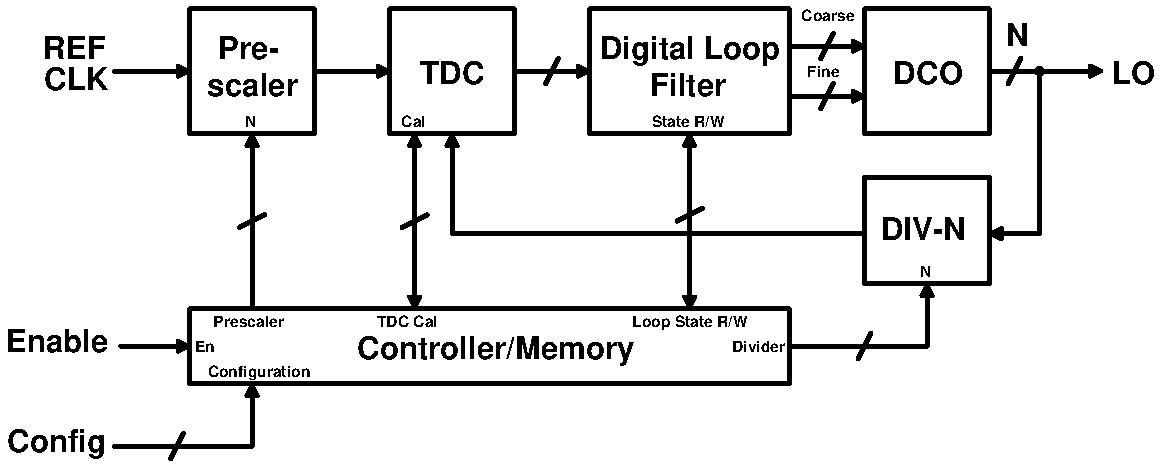
\includegraphics[width=0.75\textwidth, angle=0]{pll2.pdf}

	\end{block}
		\begin{block}{Power Targets}
		\vspace{-.1em}
		\begin{table}[htb!]
			\tiny
			\centering
			\def\arraystretch{1.5}		
			\setlength\arrayrulewidth{0.75pt}
			\setlength{\tabcolsep}{1em} % for the horizontal padding
			\begin{tabular}{|l|l|l|l|l|}
				\hline 
				\rule[-1ex]{0pt}{2.5ex} \cellcolor{gray!40}\textbf{DCO} & \cellcolor{gray!40}\textbf{TDC} & \cellcolor{gray!40}\textbf{Divider }& \cellcolor{gray!40}\textbf{Other} & \cellcolor{gray!40}\textbf{SUM} \\ 
				\hline 
				\rule[-1ex]{0pt}{2.5ex} 70 $\mu$W& 20 $\mu$W & 10 $\mu$W & $<<$ 1 $\mu$W & 100 $\mu$W\\ 
				\hline 
			\end{tabular} 
			% \caption{Assigned specifications for branch line hybrid design.}
			% \label{asgn_specs}
		\end{table}   
	\end{block}

\end{frame}


% #############################################################################
% project phases
% #############################################################################


\begin{frame}
	\frametitle{Project Phases}
	\begin{block}{Autumn 2019}
		\footnotesize
		\begin{itemize}
			\item System modeling and simulation.
			\begin{itemize}
				\footnotesize
				\item Learn PLL theory in detail
				\item Evaluate feasability of PLL architectures (counter, TDC-based)
				\item Determine requirements for TDC/DCO/Divider/logic (bits of resolution, accuracy etc) to meet PLL performance specifications.
				\item Determine digital logic for loop filter, validate stability and lock time performance.
			\end{itemize}
			\item Research ultra-low power circuit topologies to implement system components that will meet determined requirements.
			\item Translate component-level specifications into schematic-level circuit designs.
			\begin{itemize}
				\footnotesize
				\item Try, fail, try again until functional at schematic level.
				\begin{itemize}
					\footnotesize
					\item I expect the TDC to be difficult.
				\end{itemize}
			\end{itemize}      
		\end{itemize}
	\end{block}
\end{frame}

% #############################################################################
% Project phases slide 2
% #############################################################################


\begin{frame}
	\frametitle{Project Phases (continued)}
	\begin{block}{Spring 2020}
		\begin{itemize}
			\footnotesize
			\item Finalize schematic-level design.
			\item Estabilish thorough tests for PLL performance (automated?) to help in layout.
			\item Layout of PLL.
			\begin{itemize}
				\footnotesize
				\item Design iteration until design specs met.
				\item Probably very time consuming.
			\end{itemize}
			\item Full characterization/validation of design performance. 
			\begin{itemize}
				\footnotesize
				\item Comprehensive Corners/Monte-Carlo testing (time consuming??)
				\item More design iteration if new issues crop up...
			\end{itemize}
			\item Thesis paper writing.
		\end{itemize}
	\end{block}
\end{frame}

% #############################################################################
% References
% #############################################################################


% \begin{frame}
% 	\frametitle{Project Phases (continued)}
% 	\begin{block}{Spring 2020}
% 		[1] "Digital Frequency Synthesizers", Michael Perrott, 2019.\\
% 		\hspace{16pt}\url{http://www.cppsim.com/PLL_Lectures/day4_am.pdf}\\
% 		\vspace{1em}
% 		[2] "Minimum Achievable Phase Noise of RC Oscillators",
% 	Navid et al. 2005
% 	\end{block}
% \end{frame}


\end{document}
